\documentclass[tikz, margin=5mm]{standalone}
\usepackage[sfdefault,light]{roboto}
\usetikzlibrary{shapes, arrows, positioning, backgrounds}
\definecolor{MyGreen}{HTML}{41B3A3}
\tikzset{every picture/.style={/utils/exec={\sffamily}}}
\begin{document}
    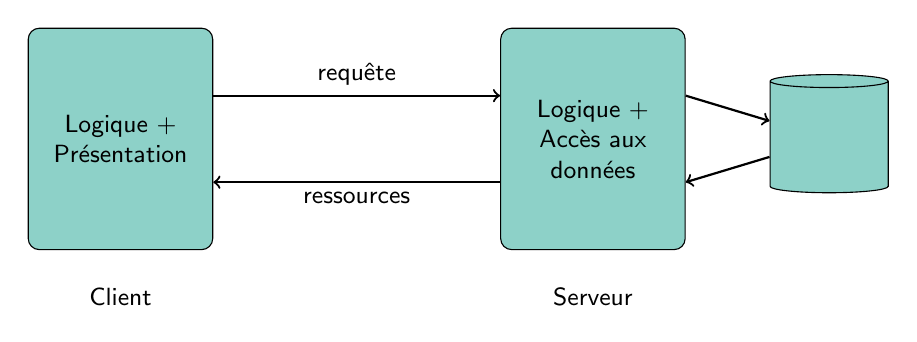
\begin{tikzpicture} [
			every node/.style={draw,font=\small,align=center},
			tier/.style={draw,rectangle,text width=60, minimum width=60, minimum height=80, fill=MyGreen!60,rounded corners},
			bdd/.style={draw,cylinder,shape border rotate=90,aspect=0.7,minimum width=15mm,minimum height=15mm, cylinder uses custom fill,cylinder body fill=MyGreen!60,cylinder end fill=MyGreen!60},
			legend/.style={draw=none,fill=none,align=center}
		]
			\node at (0,0) [tier] (nodeClient) {Logique + Présentation};
			\node at (0,-2) [legend] (legClient) {Client};
			\node at (6,0) [tier] (nodeServeur) {Logique + Accès aux données};
			\node at (6,-2) [legend] (legServeur) {Serveur};
			\node at (9,0) [bdd] (nodeBdd) {};
			\path[->, thick] (nodeClient.25) edge node [legend,above] {requête} (nodeServeur.west|-nodeClient.25);
			\path[<-, thick] (nodeClient.-25) edge node [legend,below] {ressources} (nodeServeur.west|-nodeClient.-25);
			\path[->, thick] (nodeServeur.25) edge (nodeBdd);
			\path[<-, thick] (nodeServeur.-25) edge (nodeBdd);
		\end{tikzpicture}
\end{document}